\newpage
\subsection{Technologie Diagramme}
 Hier werden die Zusammenhänge der Technologien in Form von verschiedenen Diagrammen vorgestellt.

\subsubsection{Komponentendiagramme}

\begin{figure}[H]
\centering
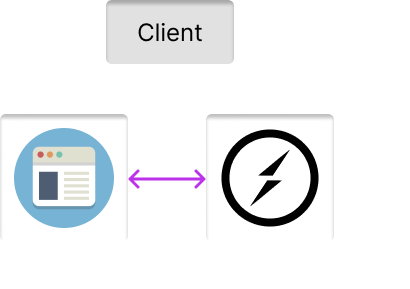
\includegraphics[width=0.5\textwidth]{bilder/technologien/KomponentendiagramClient.png}
\caption{Komponentendiagramm Client}
\label{fig:Komponentendiagramm_Client}
\end{figure}
Hier wird die Client Seite bildlich dargestellt. Man sieht, dass der Webbrowseer durch die 
Socket.io Client deployed wird und dadurch wird dann eine Beziehung zur Serverseite aufgebaut. (Siehe Abbildung \ref{fig:Komponentendiagramm_Client})

\begin{figure}[H]
\centering
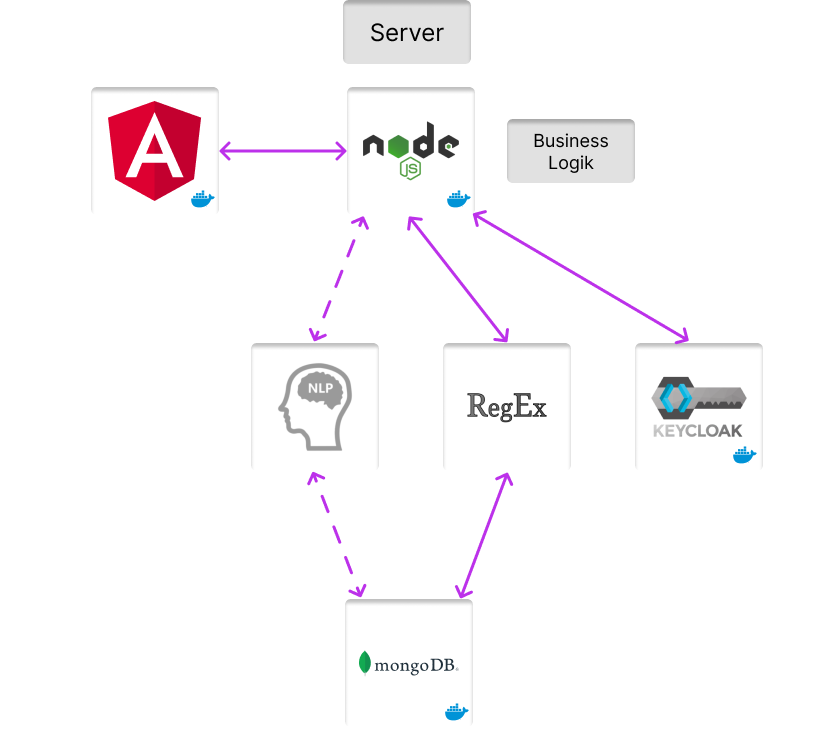
\includegraphics[width=0.9\textwidth]{bilder/technologien/KomponentendiagramServer.png}
\caption{Komponentendiagramm Server}
\label{fig:Komponentendiagramm_Server}
\end{figure}

\noindent In der Serverseite wird dann durch den Socket.io Server die Verbindug zum Clienten aufrecht gehalten.
Im Server befindet sich Angular, node.js, KeyCloak und die Datenbank mongoDB und haben jeweils einen eigenen Dockercontainer. 
Die Erkennung von der eingegeben Sprache möchten wir zunächst mit RegEx ermöglichen, 
um das Minimal Viable Product hinzubekommen. Optional dann mit NLP (Natural Language Processing) erweitern.

\begin{figure}[!hbt]
\centering
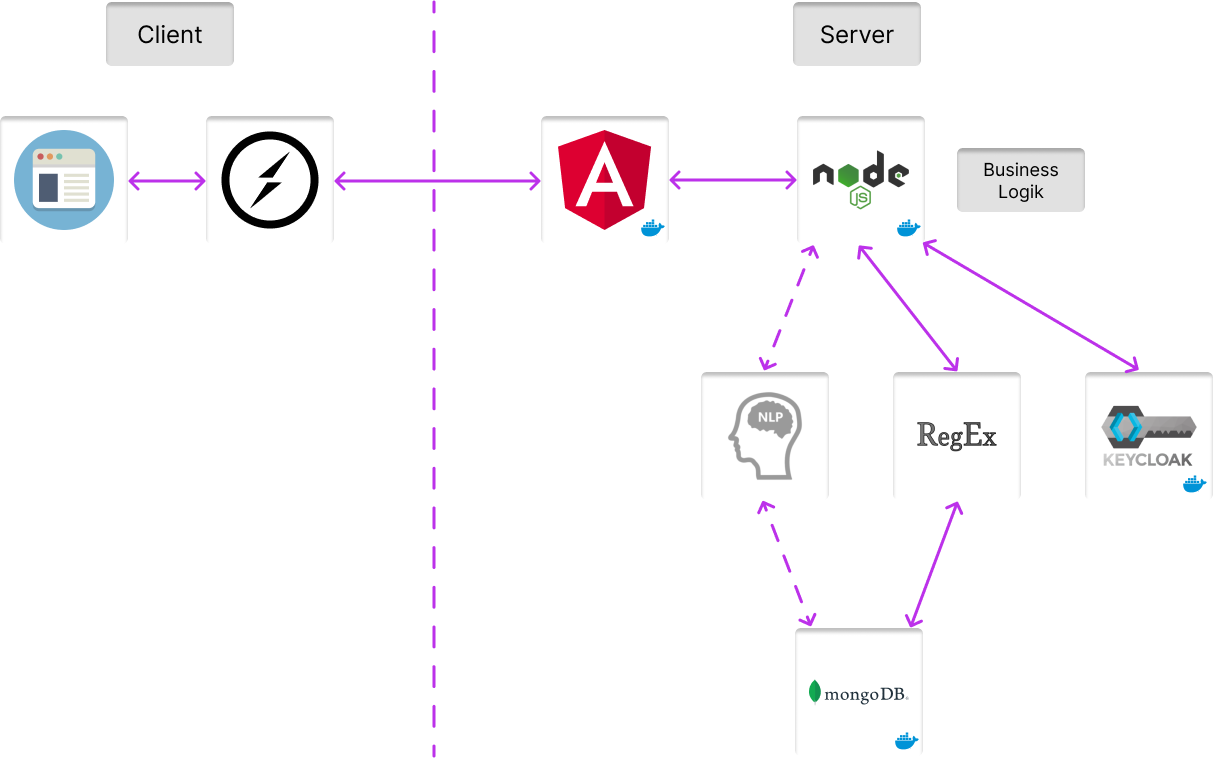
\includegraphics[width=1.0\textwidth]{bilder/technologien/Komponentendiagram v1.2.png}
\caption{Komponentendiagramm v1.2}
\label{fig:Komponentendiagramm_v1.2}
\end{figure}

\begin{figure}[!hbt]
\centering
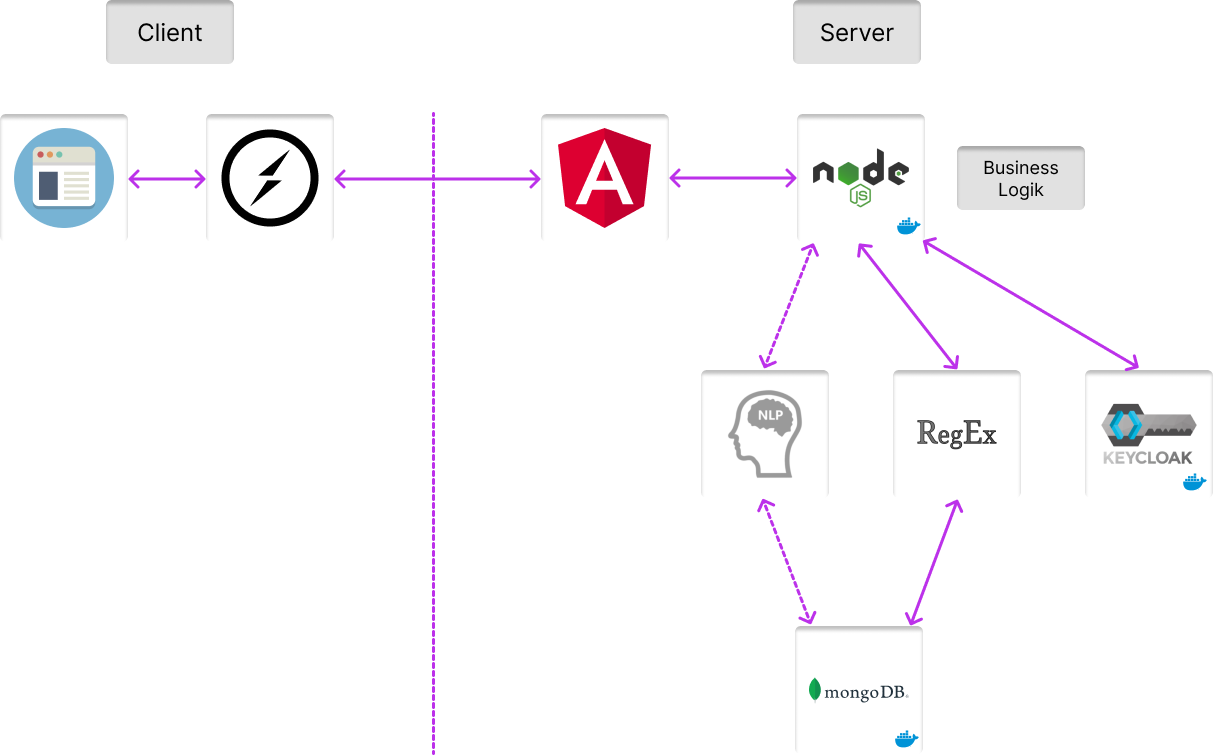
\includegraphics[width=1.0\textwidth]{bilder/technologien/Komponentendiagram v1.1.png}
\caption{Komponentendiagramm v1.1}
\label{fig:Komponentendiagramm_v1.1}
\end{figure}

\begin{figure}[!hbt]
\centering
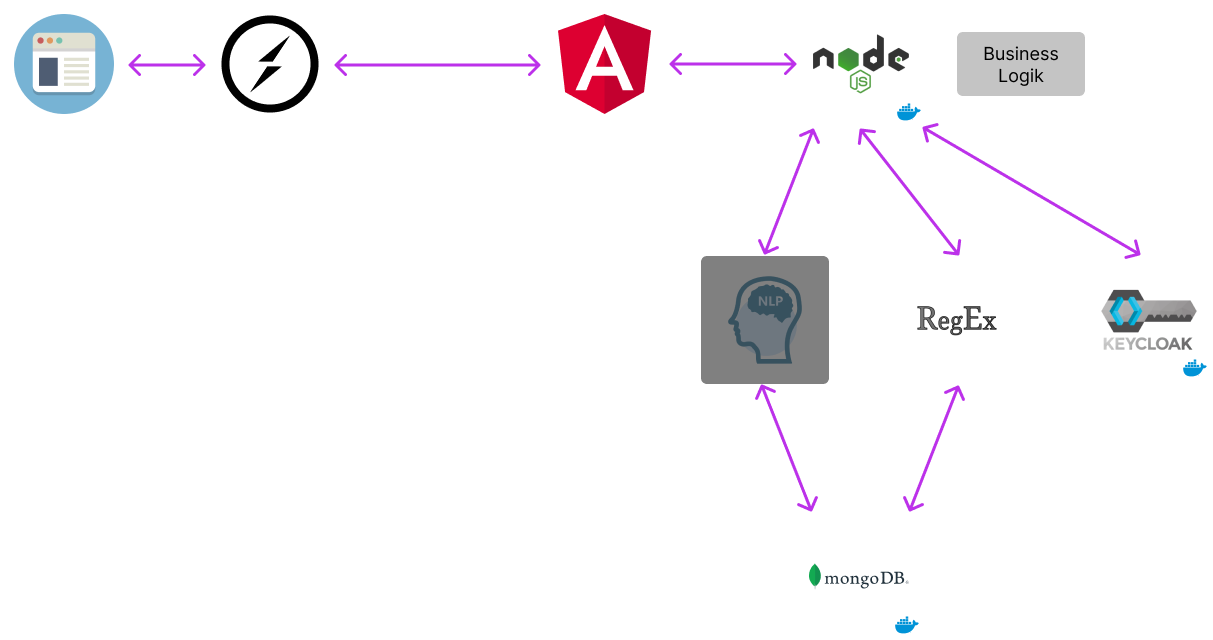
\includegraphics[width=1.0\textwidth]{bilder/technologien/Komponenten-Diagram-v1.png}
\caption{Komponentendiagramm v1.0}
\label{fig:Komponentendiagramm_v1.0}
\end{figure}
\FloatBarrier % prevent pictures from appearing under a different section

\subsubsection{Verteilungsdiagramm}

\begin{figure}[H]
\centering
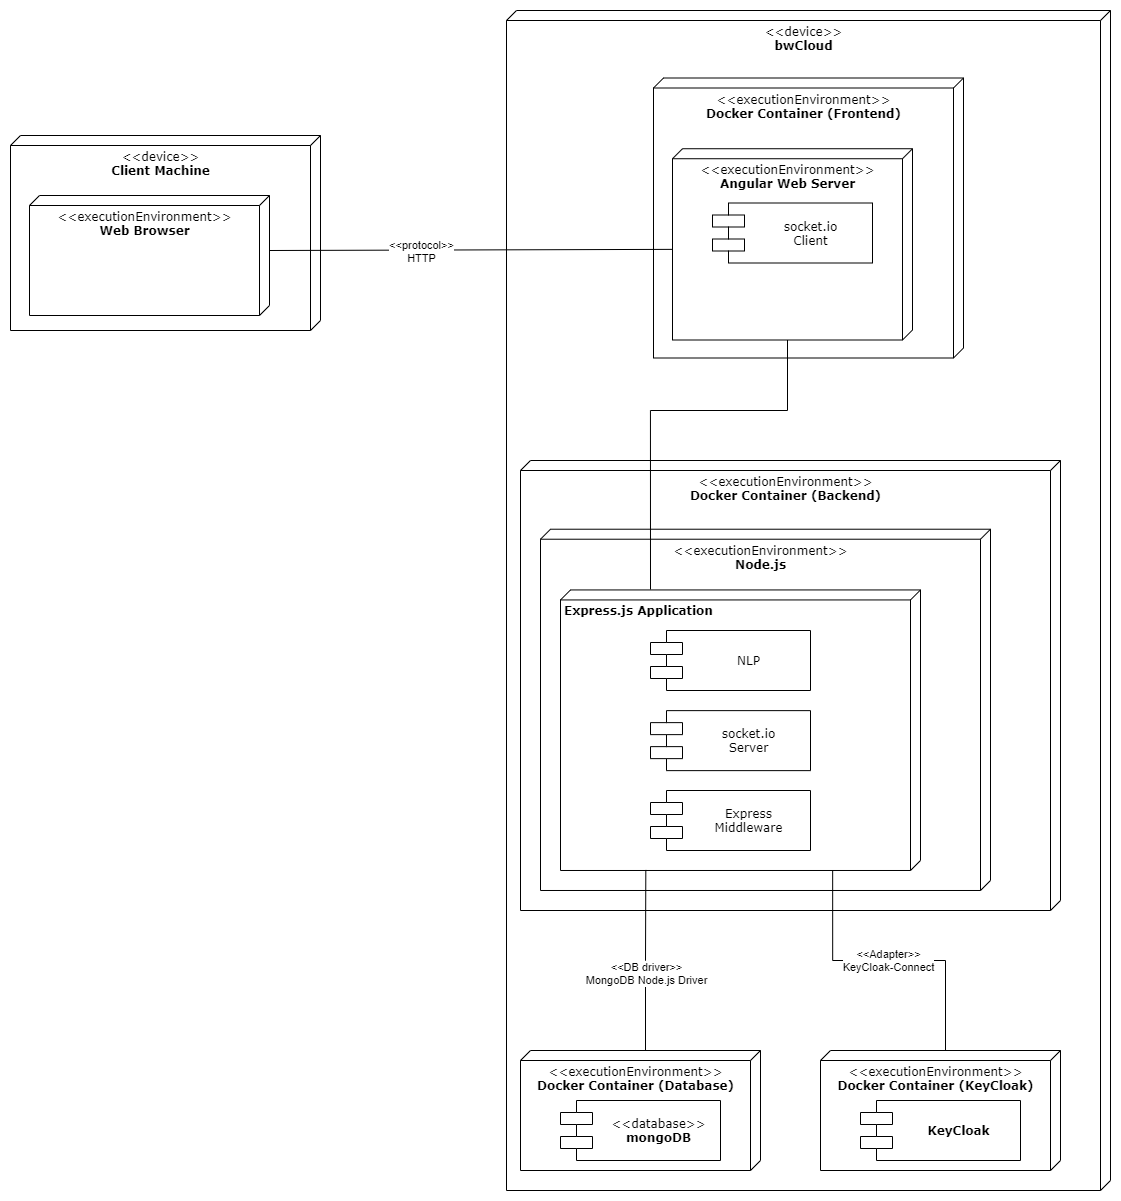
\includegraphics[width=1.0\textwidth]{bilder/technologien/Verteilunsgdiagramm.png}
\caption{Verteilungsdiagramm}
\label{fig:Verteilungsdiagramm}
\end{figure}
In unserem Verteilungsdiagramm kann man sehen, 
wie die verschiedenen Technologien verschachtelt und wie sie miteinander verbunden sind.
Außerdem kann man sehen, was wir in unsere einzelnen Dockercontainer hineinlegen.
\newline
(Siehe Abbildung \ref{fig:Verteilungsdiagramm})